\documentclass[11pt]{article}

\usepackage[margin=1in]{geometry}
\usepackage{amsmath,amssymb,bm}
\usepackage{graphicx}
\usepackage{booktabs}
\usepackage{array}
\usepackage{caption}
\usepackage{subcaption}
\usepackage{float}
\usepackage{xcolor}

\newcommand{\q}{\mathbf q}
\newcommand{\qp}{\mathbf q_p}
\newcommand{\qs}{\mathbf q_s}
\newcommand{\qbar}{\overline{\mathbf q}}
\newcommand{\V}{\mathbf V}
\newcommand{\uvec}{\mathbf u}
\newcommand{\mub}{\bm\mu}
\newcommand{\R}{\mathbf R}
\newcommand{\J}{\mathbf J}
\newcommand{\z}{\mathbf z}
\newcommand{\norm}[1]{\left\lVert #1 \right\rVert}

\title{PROM-Consistent Learned Reduced Models for a Parametric 2D Burgers Benchmark}
\author{}
\date{}

\begin{document}
\maketitle

\begin{abstract}
This manuscript studies learned reduced models at the PROM level for a two-dimensional parametric Burgers
benchmark.  A fixed MLSPG-sensitive basis of dimension \(n_{\mathrm{tot}}=151\) defines the coefficient space, and
the reference coefficient trajectories are produced by a linear PROM in that full reduced space.  We compare three
intrusive PROM--ANN closures, a PROM--POD--AE nonlinear-manifold solver, a direct POD--NN--ROM map, and a
POD--DL--ROM latent map.  Two data regimes are considered.  The baseline regime uses the original nine PROM
training trajectories.  The enriched regime keeps the same basis and the same PROM formulation, but augments the
coefficient data with 36 additional PROM trajectories selected by Latin hypercube sampling.  The enriched campaign
substantially reduces coefficient regression error and brings all learned PROM/ROM state predictions close to the
linear PROM accuracy level at the four evaluation points.  The purpose of this document is to establish a clean
PROM-consistent baseline before adding any residual-sampling approximation.
\end{abstract}

\section{Objective and Scope}
The goal is to answer a deliberately restricted question: given a fixed linear PROM space, can learned nonlinear
closures reproduce the linear PROM coefficient dynamics and state accuracy?  This is separated from online residual
sampling.  All intrusive results in this document minimize the full PROM residual, and all non-intrusive results are
reconstructed in the same \(151\)-dimensional reduced basis.

This separation is useful for two reasons.  First, it isolates the learning error from any additional quadrature or
sampling error.  Second, it makes the linear PROM coefficient trajectory a well-defined teacher for the learned
models.  If a learned model fails at this level, the failure is caused by either the learned coefficient map or by its
feedback through the nonlinear PROM solve, not by residual sampling.

\section{PROM Reference Problem}
Let \(\uvec(t;\mub)\in\mathbb R^{N_h}\) denote the HDM state for parameters
\(\mub=(\mu_1,\mu_2)\).  The reduced approximation uses the fixed affine trial space
\begin{equation}
  \uvec(t;\mub) \approx \uvec_{\mathrm{ref}} + \V_{151}\q(t;\mub),
  \qquad \V_{151}\in\mathbb R^{N_h\times151}.
  \label{eq:prom-affine-space}
\end{equation}
The basis \(\V_{151}\) is the MLSPG-sensitive basis from the current PROM campaign.  In contrast with a purely
Euclidean snapshot POD basis, this basis was selected to be compatible with the least-squares residual solve.  The
basis is fixed throughout both the baseline and enriched experiments; enrichment changes only the coefficient data
used to train the neural models.

At each time step, the linear PROM solves a least-squares residual problem in the full reduced space,
\begin{equation}
  \q_{151}^{k,\mathrm{lin}}(\mub)
  = \arg\min_{\eta\in\mathbb R^{151}}
  \left\lVert
  \R\!\left(\uvec_{\mathrm{ref}} + \V_{151}\eta;\uvec^{k-1},\mub,t_k\right)
  \right\rVert_2^2 .
  \label{eq:linear-prom-lspg}
\end{equation}
The resulting trajectory \(\q_{151}^{\mathrm{lin}}(t;\mub)\) is used as the coefficient reference for training and
for coefficient-space diagnostics.  State errors are always measured against the HDM snapshots,
\begin{equation}
  e_u(\mub) = 100\,\frac{\norm{\uvec_{\mathrm{HDM}}-\uvec_{\mathrm{ROM}}}_F}
  {\norm{\uvec_{\mathrm{HDM}}}_F} .
\end{equation}
Coefficient errors are measured against the linear PROM teacher,
\begin{equation}
  e_q(\mub) = 100\,\frac{\norm{\q^{\mathrm{lin}}_{151}-\widehat{\q}}_F}
  {\norm{\q^{\mathrm{lin}}_{151}}_F} .
\end{equation}

\section{Learned Model Families}
The learned models all use the same fixed coefficient space, but differ in which coordinates are solved by the PROM
residual and which coordinates are predicted.

\paragraph{PROM--ANN Case 1.}
The PROM solves the first ten coordinates \(\qp=(q_1,\ldots,q_{10})\).  The secondary coordinates
\(\qs=(q_{11},\ldots,q_{151})\) are predicted from the solved primary coordinates,
\begin{equation}
  \qs = \mathcal N_1(\qp).
  \label{eq:case1}
\end{equation}
This closure is state-only.  It is intrusive because \(\qp\) is determined by a residual minimization, but it does
not receive \(\mub\) or \(t\) explicitly.

\paragraph{PROM--ANN Case 2 and POD--NN--ROM.}
A master map predicts the full coefficient vector from parameters and time,
\begin{equation}
  \widehat{\q}_{151}=\mathcal N_2(\mu_1,\mu_2,t).
  \label{eq:master-map}
\end{equation}
The same map is used in two ways.  With \(n=0\), it is the purely non-intrusive POD--NN--ROM.  With
\(0<n<151\), the PROM solves \((q_1,\ldots,q_n)\) by least squares and injects the tail
\((\widehat q_{n+1},\ldots,\widehat q_{151})\) from the master map.  With \(n=151\), the method becomes the
linear PROM in Eq.~\eqref{eq:linear-prom-lspg}.

\paragraph{PROM--ANN Case 3.}
The PROM again solves \(\qp=(q_1,\ldots,q_{10})\), but the secondary closure receives both the solved primary
coordinates and the parameter--time coordinates,
\begin{equation}
  \qs = \mathcal N_3(\qp,\mu_1,\mu_2,t).
  \label{eq:case3}
\end{equation}
This is the most informative ANN closure among Cases 1--3 because it combines residual-solved coordinates with
explicit parametric context.

\paragraph{PROM--POD--AE.}
An autoencoder is trained on the linear PROM coefficient trajectories.  Its decoder defines a nonlinear coefficient
manifold,
\begin{equation}
  \q_{151}\approx\mathcal D(\z), \qquad \z\in\mathbb R^{10}.
  \label{eq:podae}
\end{equation}
The online unknown is \(\z\), and the PROM residual is minimized over this latent coordinate.

\paragraph{POD--DL--ROM.}
The POD--DL--ROM is non-intrusive.  It learns a map from \((\mu_1,\mu_2,t)\) to a latent coordinate \(\z\), then
decodes \(\z\) to \(\q_{151}\).  This tests whether the parameter--time map is easier in a learned latent space
than in all 151 coefficients.

\section{Data Sets and Evaluation Points}
The baseline training set is the original \(3\times3\) parameter grid, giving nine PROM coefficient trajectories.
Two additional PROM trajectories are used only as external validation data for the parameter--time networks; these
validation points are not part of the four test points reported below.  The four evaluation points are
\begin{align*}
  \mub^{(v)} &= (4.875,0.0225), &
  \mub^{(1)} &= (4.560,0.0190),\\
  \mub^{(2)} &= (5.190,0.0260), &
  \mub^{(3)} &= (4.000,0.0330).
\end{align*}
Here \(\mub^{(v)}\) is the verification point, \(\mub^{(1)}\) and \(\mub^{(2)}\) are off-grid in-domain points, and
\(\mub^{(3)}\) is an extrapolatory point.

The enriched data set keeps the same basis \(\V_{151}\) and the same PROM solver, but adds coefficient trajectories
at 36 new parameter points.  Eighteen are interior Latin-hypercube samples in the original training rectangle, and
18 are exterior Latin-hypercube samples in a rectangle expanded by a 25\% margin.  The LHS seed is fixed to 42.
No additional HDM snapshots are used to train these coefficient maps; the additional targets are generated by the
linear PROM teacher.

\begin{table}[H]
\centering
\caption{PROM coefficient data used for the enriched training campaign.}
\label{tab:prom-enrichment-dataset}
\begin{tabular}{lr}
\toprule
Quantity & Value \\ 
\midrule
Baseline PROM trajectories & 9 \\ 
Interior LHS trajectories & 18 \\ 
Exterior LHS trajectories & 18 \\ 
Total training trajectories & 45 \\ 
Snapshots per trajectory & 501 \\ 
Training samples & 22545 \\ 
LHS seed & 42 \\ 
Margin fraction & 0.25 \\ 
\bottomrule
\end{tabular}

\end{table}

\begin{figure}[H]
\centering
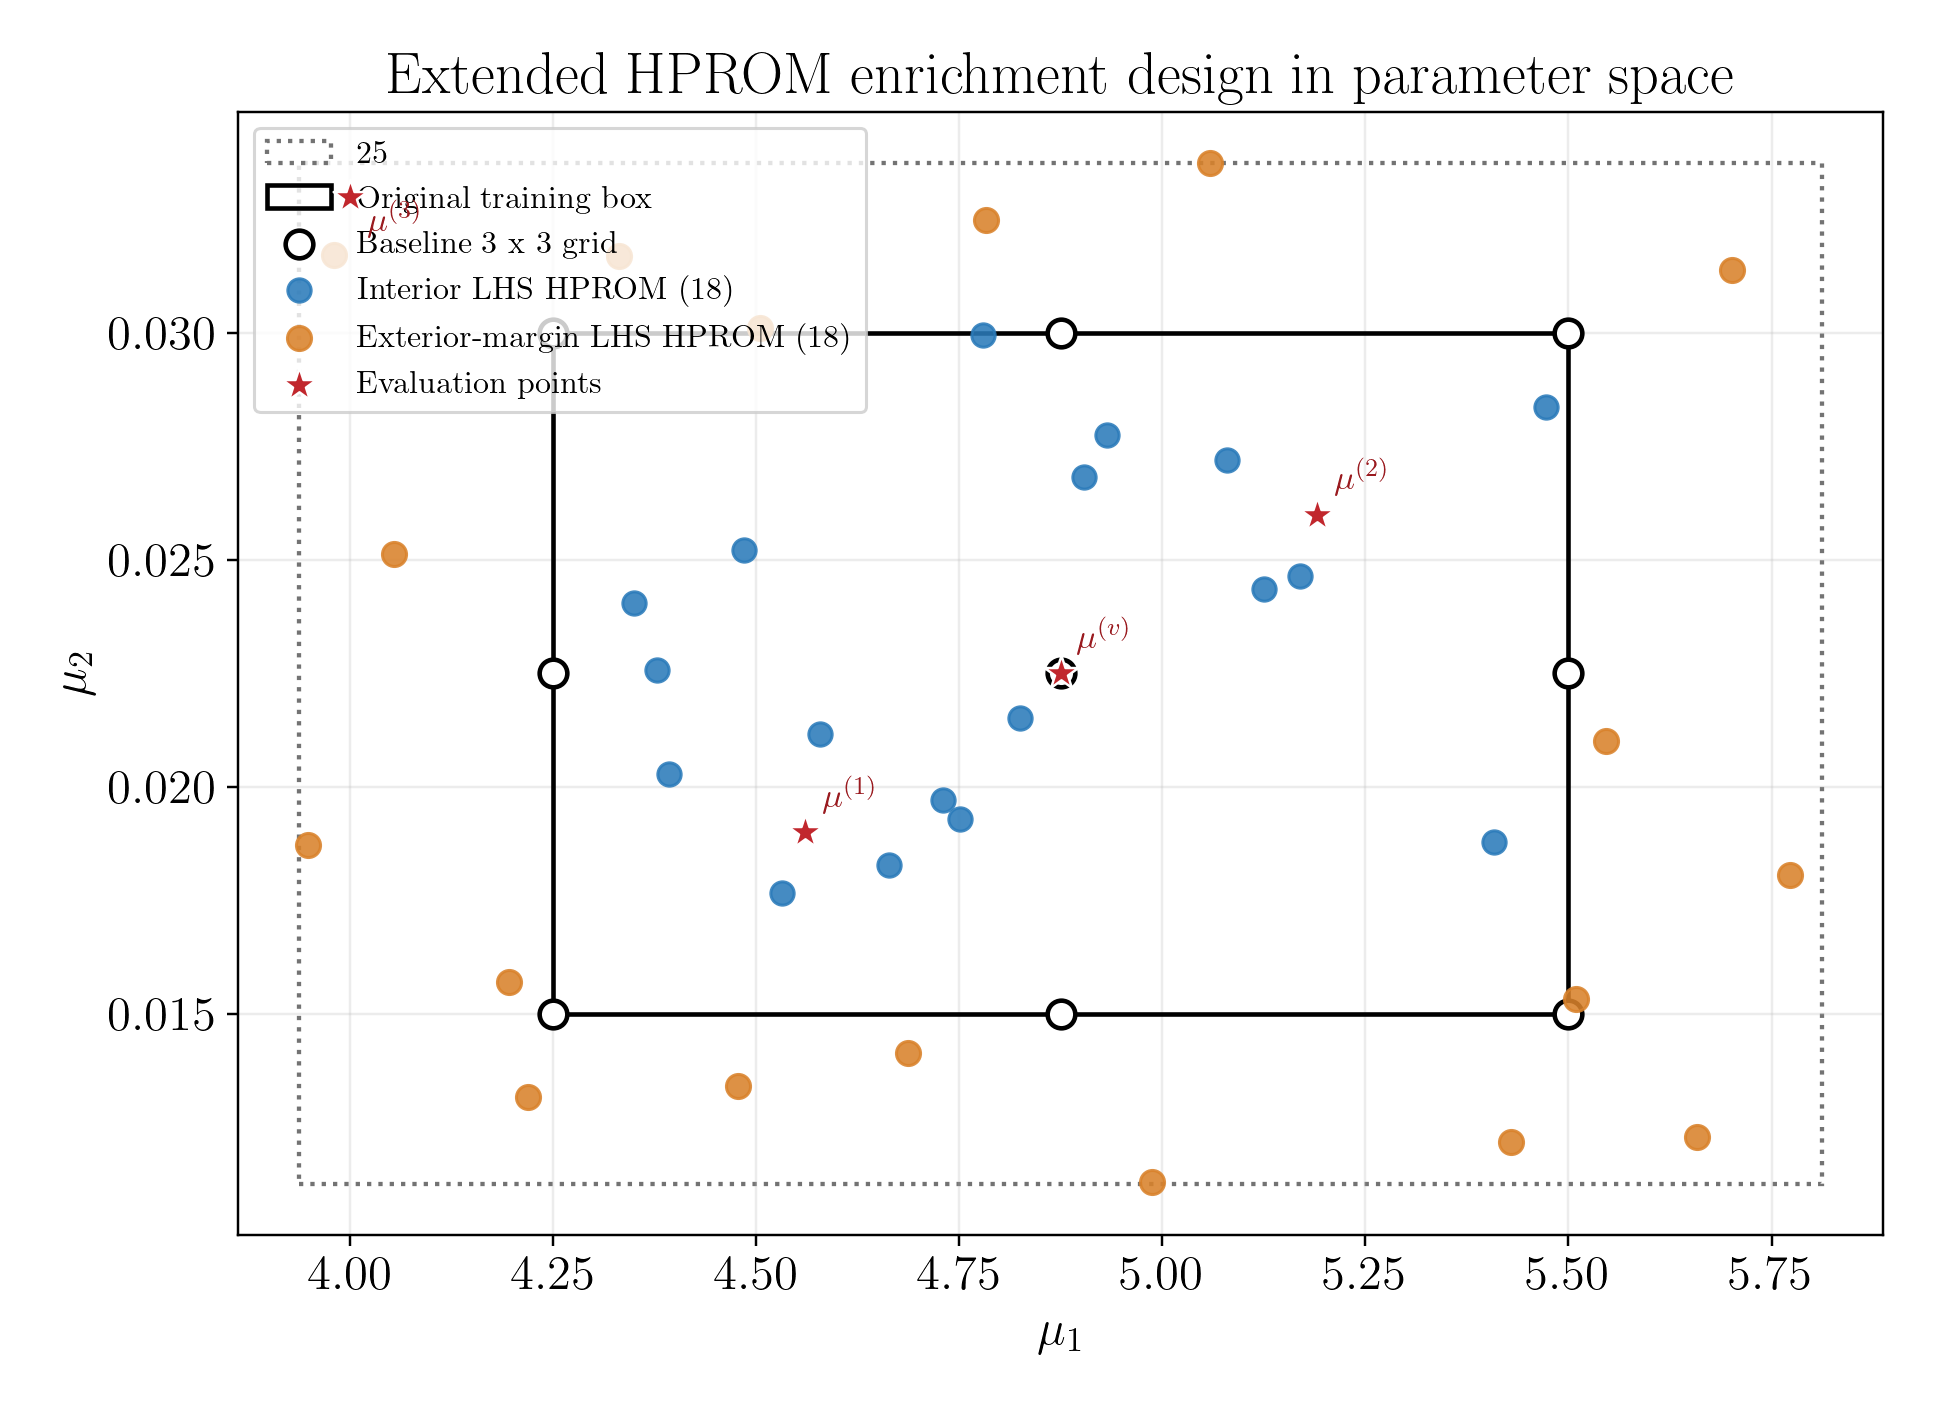
\includegraphics[width=0.72\textwidth]{Figures/prom_only/prom_enrichment_sampling_points.png}
\caption{Parameter locations for the enriched PROM coefficient data set.  The 36 additional trajectories are used
only for training the learned maps; the four reported evaluation points remain unchanged.}
\label{fig:prom-enrichment-sampling}
\end{figure}

\section{Baseline PROM-Only Results}
Table~\ref{tab:prom-training} reports the selected baseline training runs.  The largest validation error occurs for
the master parameter--time map because it predicts all 151 coefficients from only \((\mu_1,\mu_2,t)\).  The Case 1,
Case 3, and autoencoder tasks are easier because their inputs contain coefficient information.

\begin{table}[H]
\centering
\caption{Baseline PROM-only Stage--3 selected networks.  Errors are relative Frobenius percentages in coefficient space.}
\label{tab:prom-training}
\resizebox{\textwidth}{!}{\begin{tabular}{llrrr}
\toprule
Model & learned map & parameters & train (\%) & validation (\%) \\
\midrule
PROM--ANN Case 1 & $(q_1,\ldots,q_{10})\mapsto(q_{11},\ldots,q_{151})$ & 564,621 & 1.130 & 1.251 \\
PROM--ANN Case 3 & $(q_1,\ldots,q_{10},\mu_1,\mu_2,t)\mapsto(q_{11},\ldots,q_{151})$ & 565,389 & 0.405 & 0.482 \\
Master POD--NN--ROM (Case 2 tail source) & $(\mu_1,\mu_2,t)\mapsto(q_1,\ldots,q_{151})$ & 565,399 & 2.601 & 4.391 \\
PROM--POD--AE & $q_{1:151}\mapsto z_{1:10}\mapsto q_{1:151}$ & 486,817 & 0.106 & 0.127 \\
POD--DL--ROM & $(\mu_1,\mu_2,t)\mapsto z_{1:10}\mapsto q_{1:151}$ & 952,747 & 0.810 & 0.935 \\
\bottomrule
\end{tabular}
}
\end{table}

Table~\ref{tab:prom-online} gives the baseline online state error.  The linear PROM is not a theorem-level lower
bound against the HDM, but it is the reference accuracy level associated with the fixed \(151\)-dimensional PROM
basis and teacher data.  The intrusive learned PROMs are close to that reference for in-domain points.  The purely
non-intrusive maps degrade more strongly, especially at the extrapolatory point.

\begin{table}[H]
\centering
\caption{Baseline PROM-only online errors
\(100\norm{\uvec_{\mathrm{HDM}}-\uvec_{\mathrm{ROM}}}_F/\norm{\uvec_{\mathrm{HDM}}}_F\).  The mean column averages
\(\mub^{(v)},\mub^{(1)},\mub^{(2)}\).}
\label{tab:prom-online}
\resizebox{\textwidth}{!}{\begin{tabular}{lrrrrr}
\toprule
Model & $\mu^{(v)}$ & $\mu^{(1)}$ & $\mu^{(2)}$ & Mean & $\mu^{(3)}$ \\
\midrule
Linear PROM & 0.413 & 0.460 & 0.472 & 0.448 & 0.868 \\
PROM--ANN Case 1 & 0.409 & 0.520 & 0.683 & 0.537 & 1.584 \\
PROM--ANN Case 2 ($n=10$) & 1.013 & 1.427 & 1.670 & 1.370 & 1.898 \\
PROM--ANN Case 2 ($n=20$) & 0.999 & 1.328 & 1.505 & 1.278 & 1.658 \\
PROM--ANN Case 3 & 0.405 & 0.521 & 0.576 & 0.501 & 1.392 \\
PROM--POD--AE ($n_z=10$) & 0.408 & 0.539 & 0.607 & 0.518 & 1.978 \\
\midrule
POD--NN--ROM & 1.036 & 1.675 & 1.842 & 1.518 & 3.214 \\
POD--DL--ROM ($n_z=10$) & 0.489 & 1.398 & 1.463 & 1.116 & 3.728 \\
\bottomrule
\end{tabular}
}
\end{table}

\begin{figure}[H]
\centering
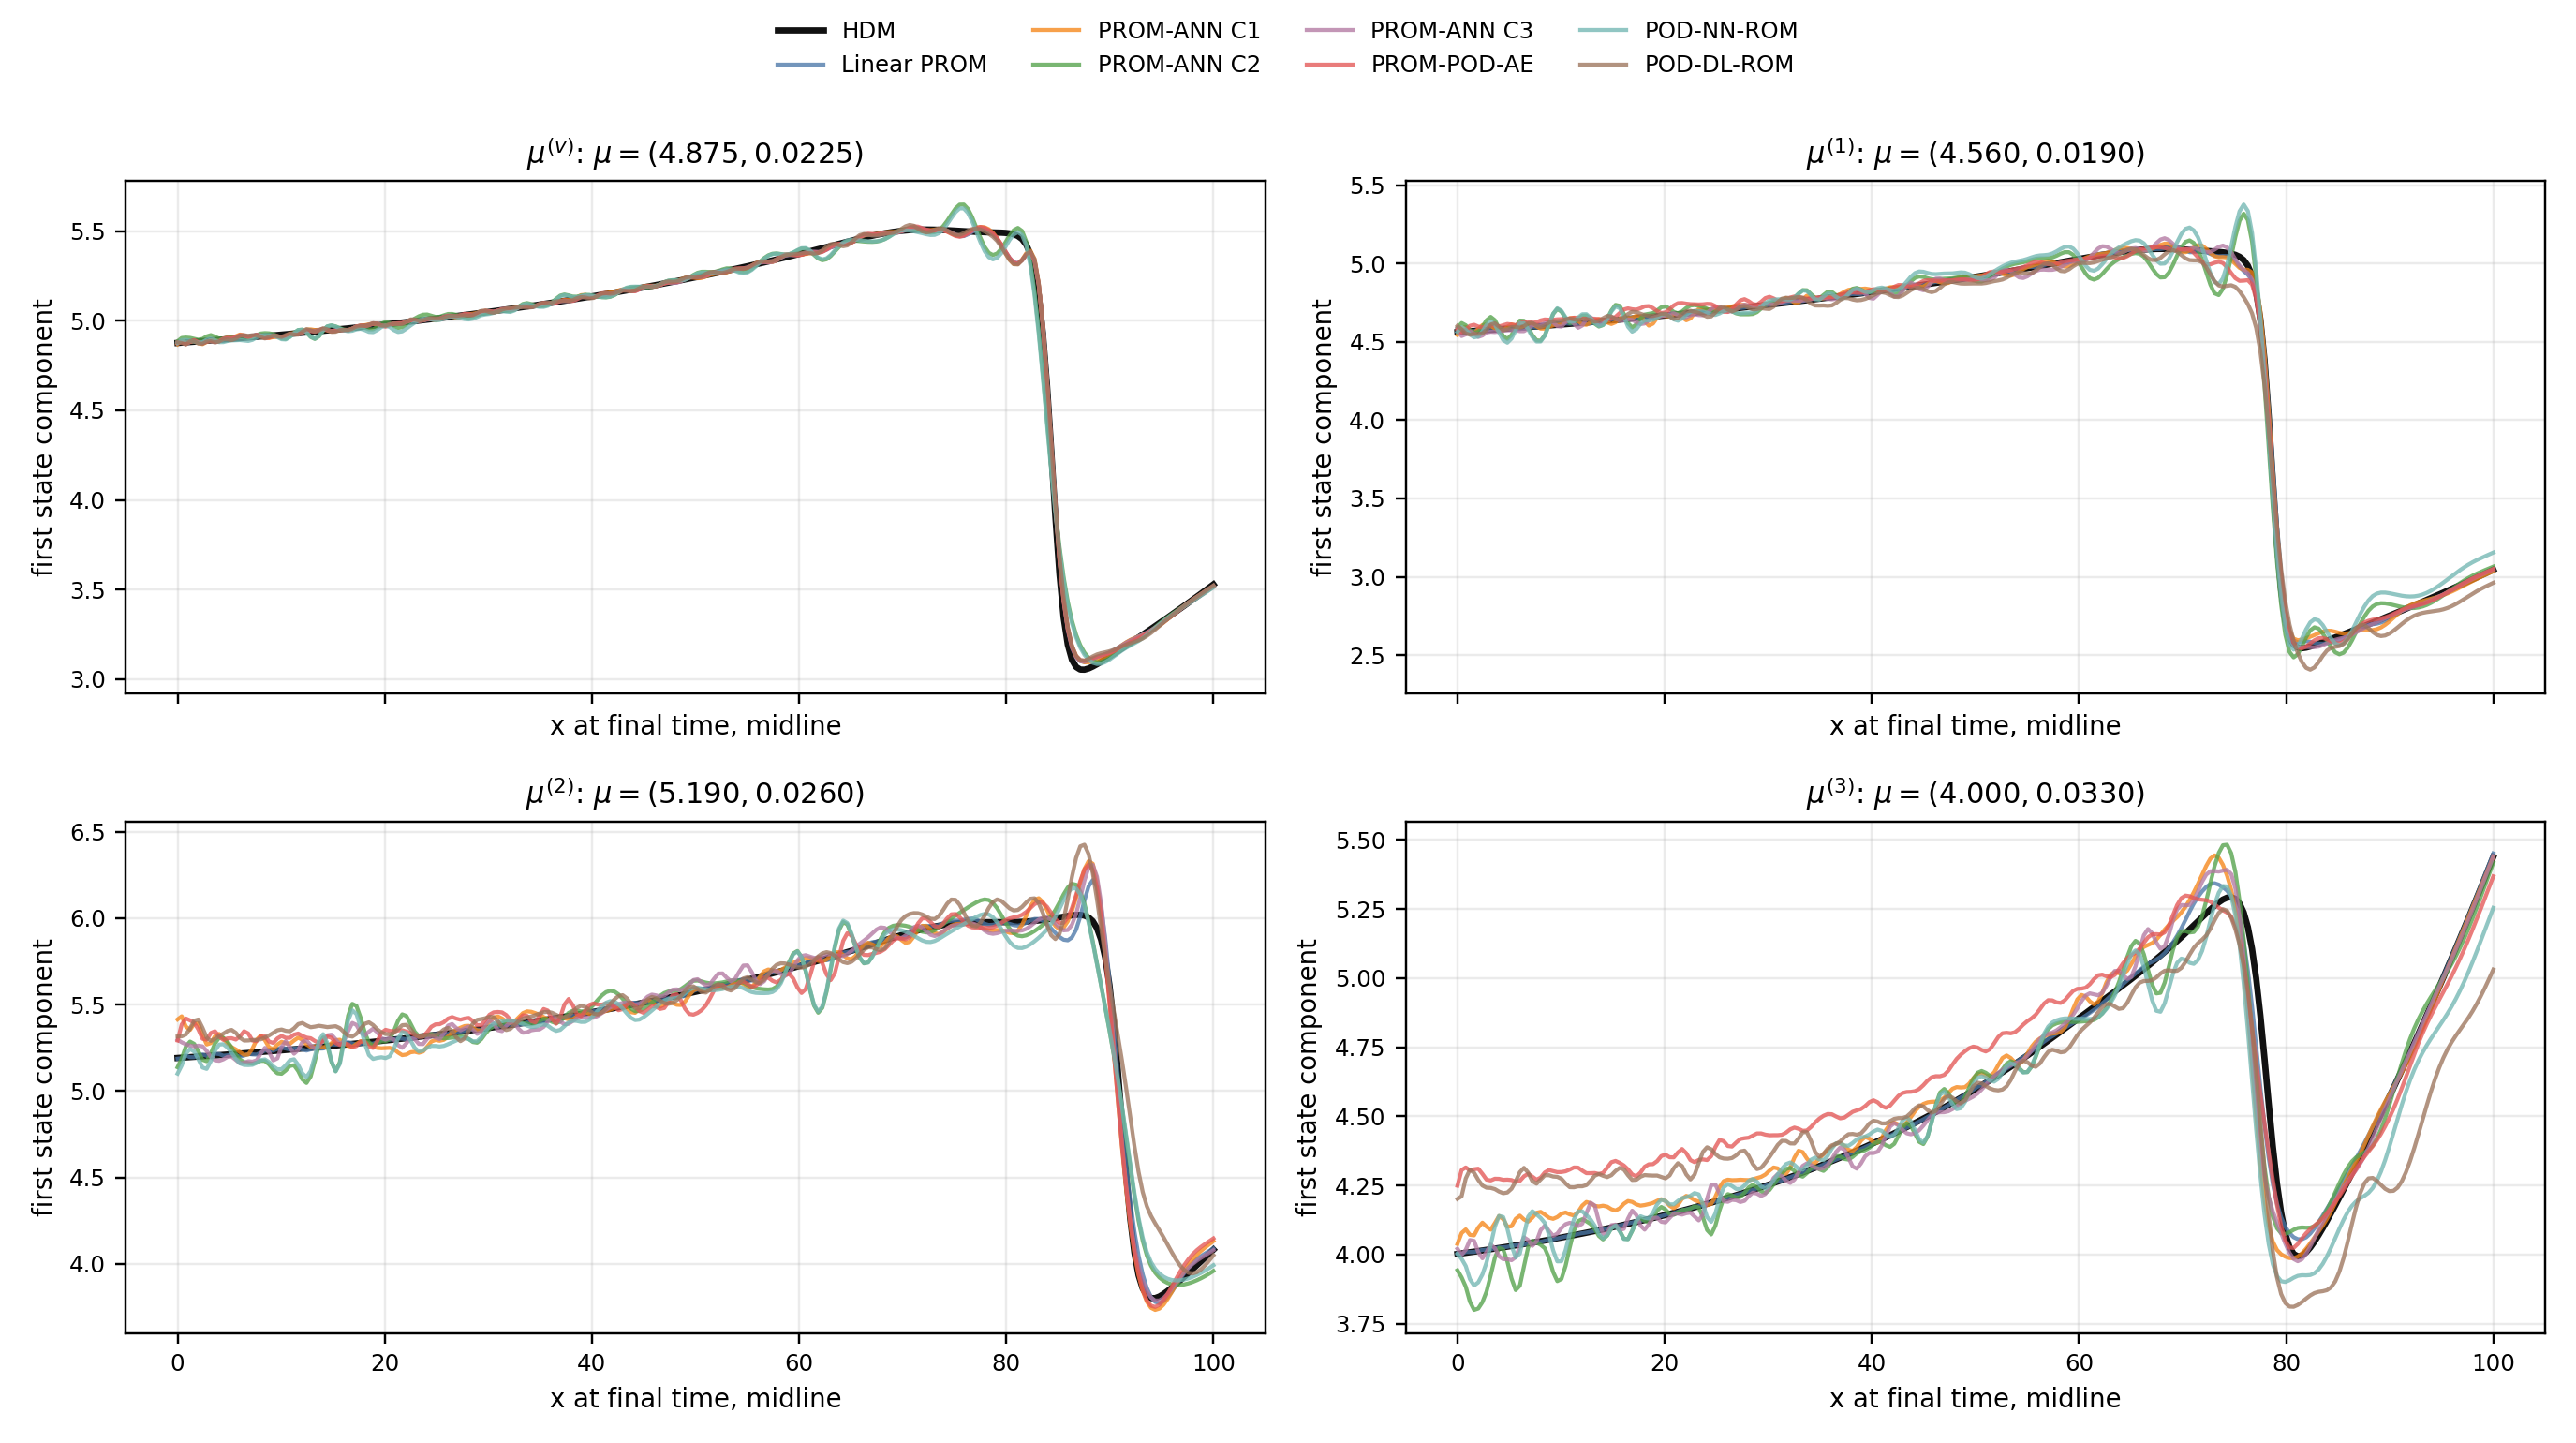
\includegraphics[width=0.98\textwidth]{Figures/prom_only/prom_only_solution_overlays.png}
\caption{Baseline PROM-only final-time midline comparison against the HDM at the four evaluation points.  All
curves are computed from saved solver-side snapshots.}
\label{fig:prom-solution-overlays}
\end{figure}

\section{Case 2 Mechanism: From POD--NN--ROM to Linear PROM}
Case 2 gives a useful diagnostic because it connects the direct parameter--time map to the full linear PROM.  We run
\begin{equation}
  n\in\{0,3,5,10,20,30,50,100,151\},
\end{equation}
where \(n=0\) is the POD--NN--ROM prediction and \(n=151\) is the linear PROM.  For intermediate \(n\), LSPG solves
the first \(n\) coordinates while the master ANN supplies the remaining coordinates.

\begin{figure}[H]
\centering
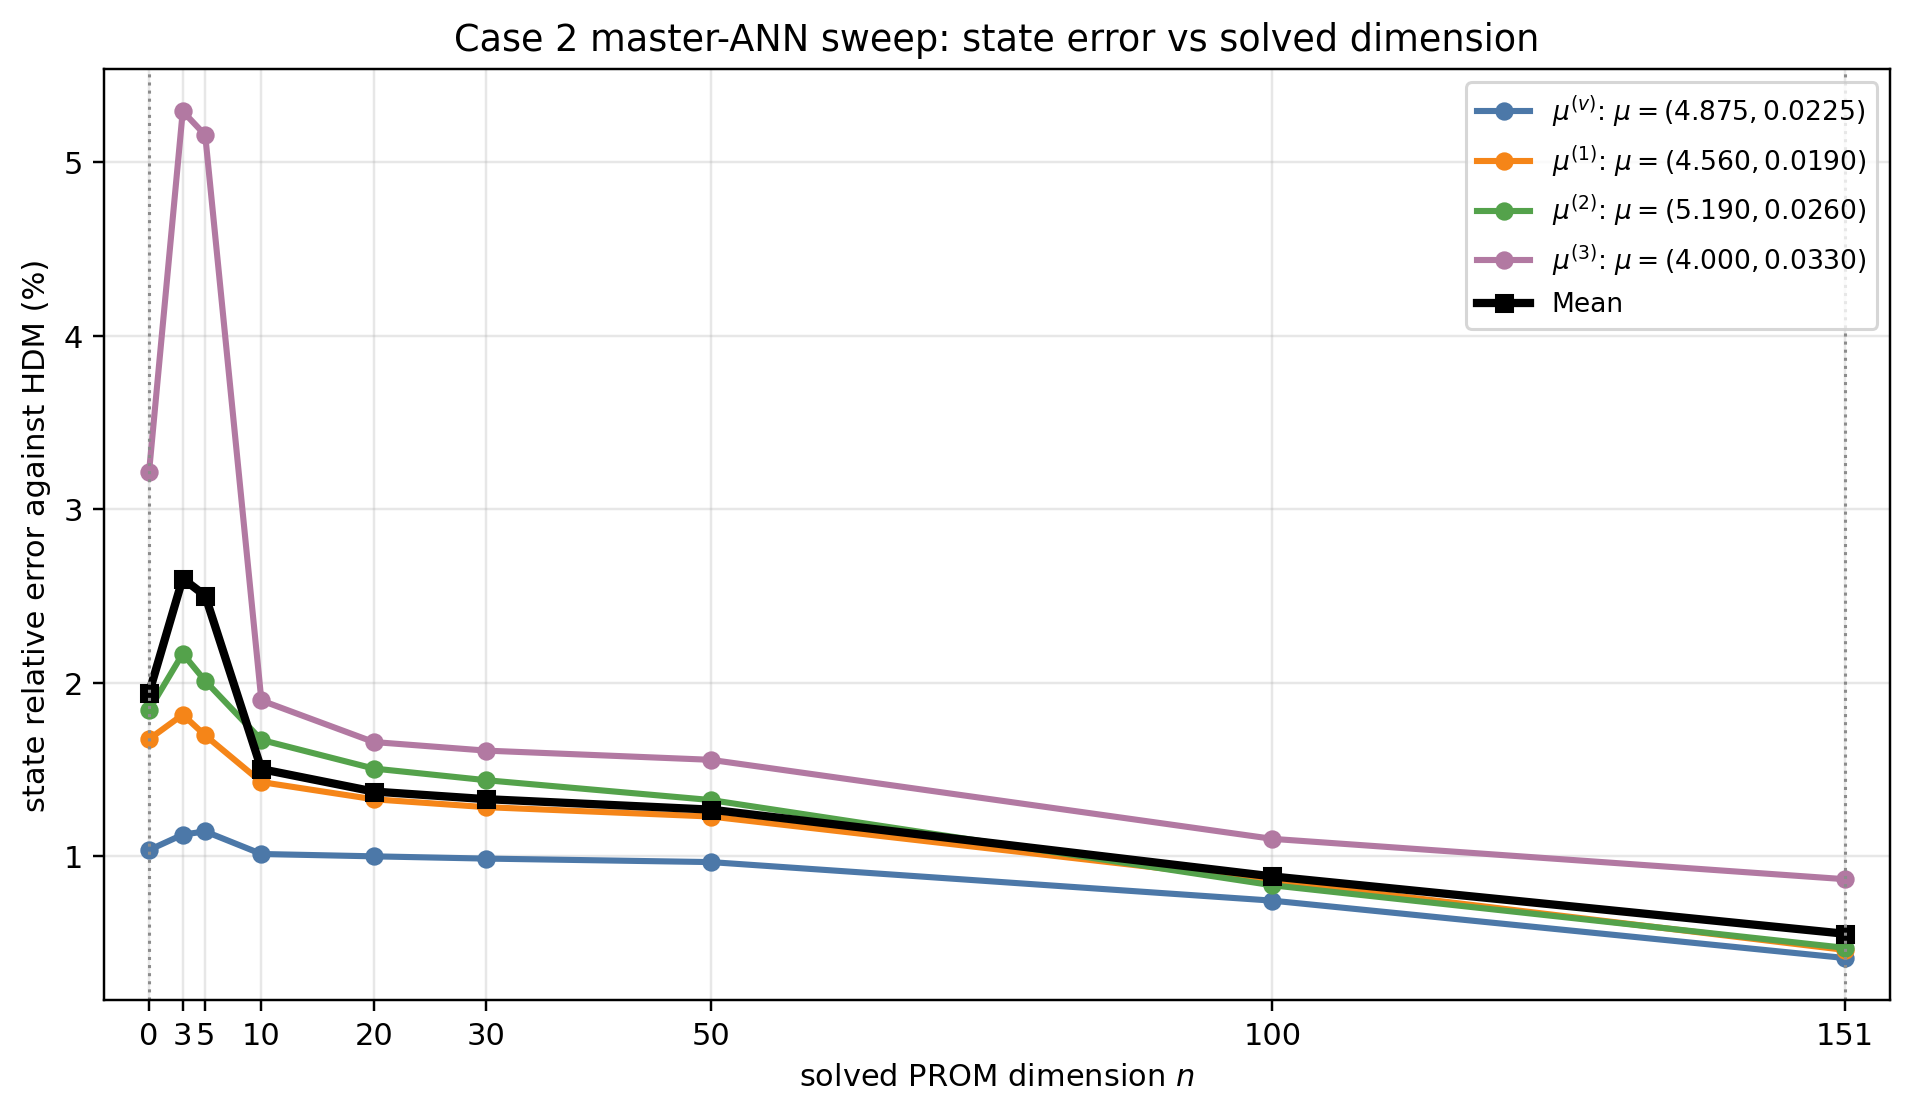
\includegraphics[width=0.88\textwidth]{Figures/prom_only/prom_case2_n_sweep_state_errors.png}
\caption{Baseline Case 2 state error as a function of the number of solved primary coordinates.  The left endpoint
is the direct POD--NN--ROM map and the right endpoint is the linear PROM.}
\label{fig:prom-case2-n-sweep-state}
\end{figure}

The sweep shows that solving more primary coordinates does not automatically produce monotone improvement at all
points.  The injected tail still affects the residual minimization, and the benefit of increasing \(n\) depends on
whether the remaining predicted tail is accurate enough for that parameter point.

\begin{figure}[H]
\centering
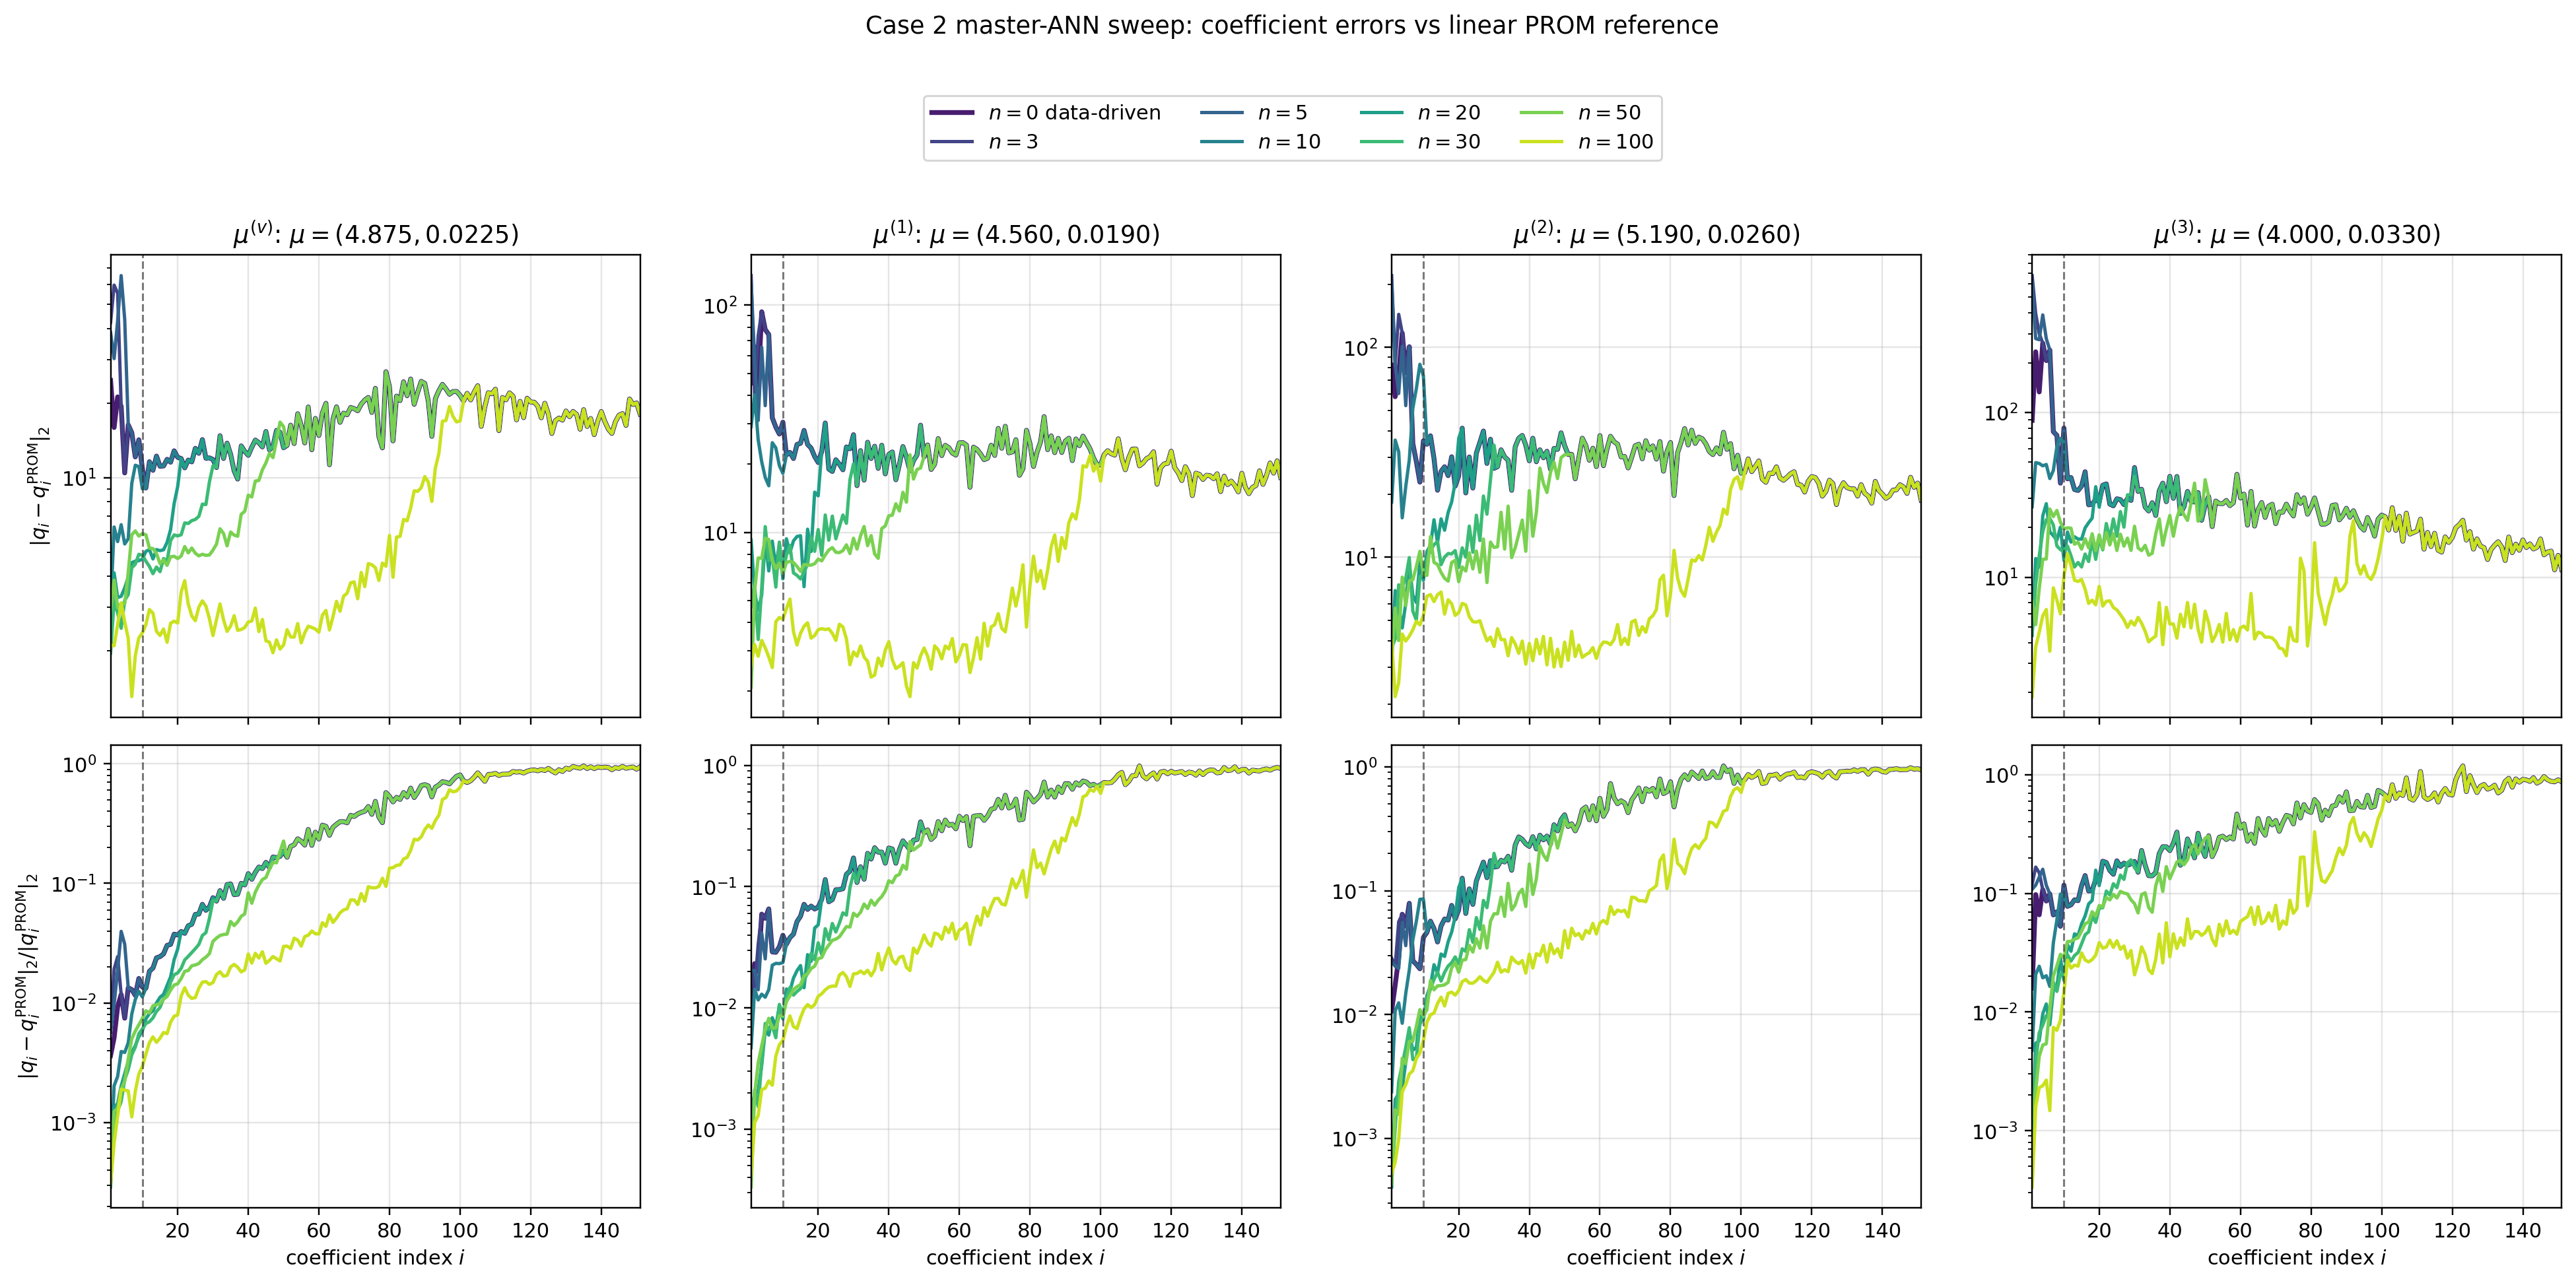
\includegraphics[width=0.98\textwidth]{Figures/prom_only/prom_case2_n_sweep_coeff_abs_rel_all_points.png}
\caption{Baseline Case 2 coefficient errors with respect to the linear PROM coefficient trajectories for the same
\(n\)-sweep.  The vertical line marks coefficient 10, the primary dimension used in the main Case 2 runs.}
\label{fig:prom-case2-n-sweep-coeff}
\end{figure}

To separate the role of the injected secondary coordinates from the LSPG solve itself, we also perturb the secondary
coordinates around the linear PROM values for the fixed \(n=10\) split.  This diagnostic asks how much
primary-coordinate and state error is induced when the secondary tail is no longer exact.

\begin{figure}[H]
\centering
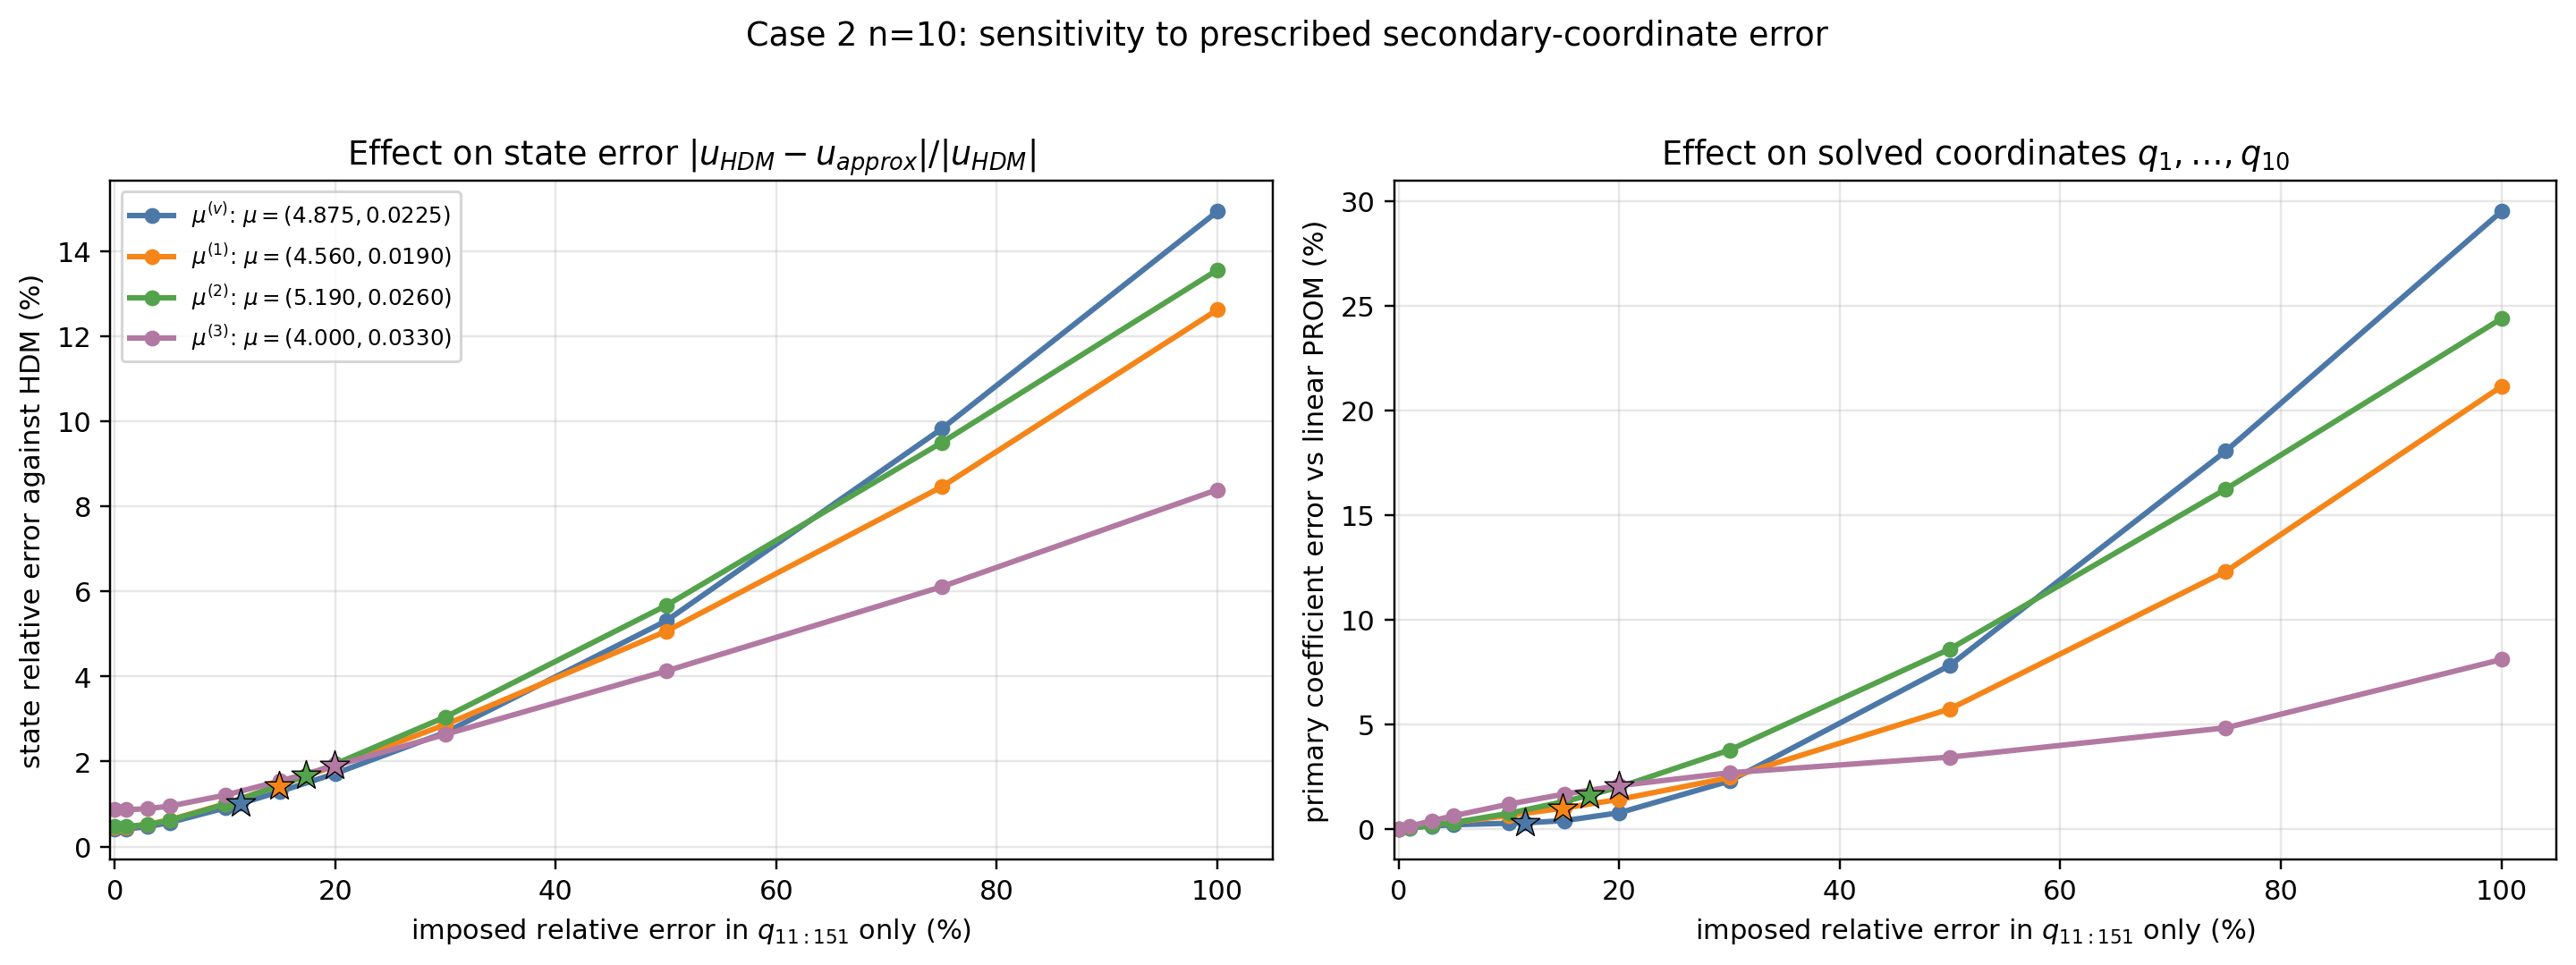
\includegraphics[width=0.95\textwidth]{Figures/prom_only/case2_secondary_sensitivity_state_and_primary_error.png}
\caption{Baseline Case 2 secondary-coordinate perturbation diagnostic for \(n=10\).  The imposed
secondary-coordinate error is measured relative to the linear PROM tail; the output curves report the induced state
and primary-coordinate errors.}
\label{fig:prom-case2-secondary-sensitivity}
\end{figure}

The interpretation is that Case 2 is not only a regression problem for the tail.  Tail errors can change the solved
primary coordinates, so the online error reflects both tail-prediction error and residual-solve feedback.

\section{Baseline Online Coefficient Diagnostics}
The online state error is the final metric, but coefficient-space diagnostics explain where the learned models lose
accuracy.  Table~\ref{tab:prom-online-coeff} reports coefficient errors from the actual online outputs.  Case 1,
Case 2, Case 3, and PROM--POD--AE use their PROM online trajectories, while POD--NN--ROM and POD--DL--ROM use their
direct non-intrusive predictions.  All coefficient errors are measured against the linear PROM trajectory with
\(n_{\mathrm{tot}}=151\).  For Case 1 and Case 3, the online solver did not save \(\q(t)\) directly, so the
coefficients are recovered from the saved PROM state snapshots by
\begin{equation}
  \q(t)=\arg\min_{\eta\in\mathbb R^{151}}
  \left\lVert \V_{151}\eta-\left(\uvec_{\mathrm{PROM}}(t)-\uvec_{\mathrm{ref}}\right)\right\rVert_2 .
\end{equation}

\begin{table}[H]
\centering
\caption{Baseline online coefficient error against the linear PROM with \(n_{\mathrm{tot}}=151\).  Values are
relative Frobenius percentages over all 151 coefficients and all time steps.}
\label{tab:prom-online-coeff}
\resizebox{0.9\textwidth}{!}{\begin{tabular}{lrrrrr}
\toprule
Model & $\mu^{(v)}$ & $\mu^{(1)}$ & $\mu^{(2)}$ & Mean & $\mu^{(3)}$ \\
\midrule
Linear PROM & 0.000 & 0.000 & 0.000 & 0.000 & 0.000 \\
PROM--ANN Case 1 & 0.295 & 0.593 & 1.297 & 0.729 & 2.923 \\
PROM--ANN Case 2 ($n=10$) & 2.440 & 3.361 & 3.906 & 3.236 & 4.257 \\
PROM--ANN Case 2 ($n=20$) & 2.401 & 3.123 & 3.512 & 3.012 & 3.662 \\
PROM--ANN Case 3 & 0.164 & 0.856 & 0.788 & 0.603 & 2.396 \\
PROM--POD--AE & 0.140 & 0.773 & 0.929 & 0.614 & 4.394 \\
\midrule
POD--NN--ROM & 2.499 & 3.924 & 4.249 & 3.557 & 7.444 \\
POD--DL--ROM & 0.814 & 3.129 & 3.225 & 2.389 & 8.639 \\
\bottomrule
\end{tabular}
}
\end{table}

\begin{figure}[H]
\centering
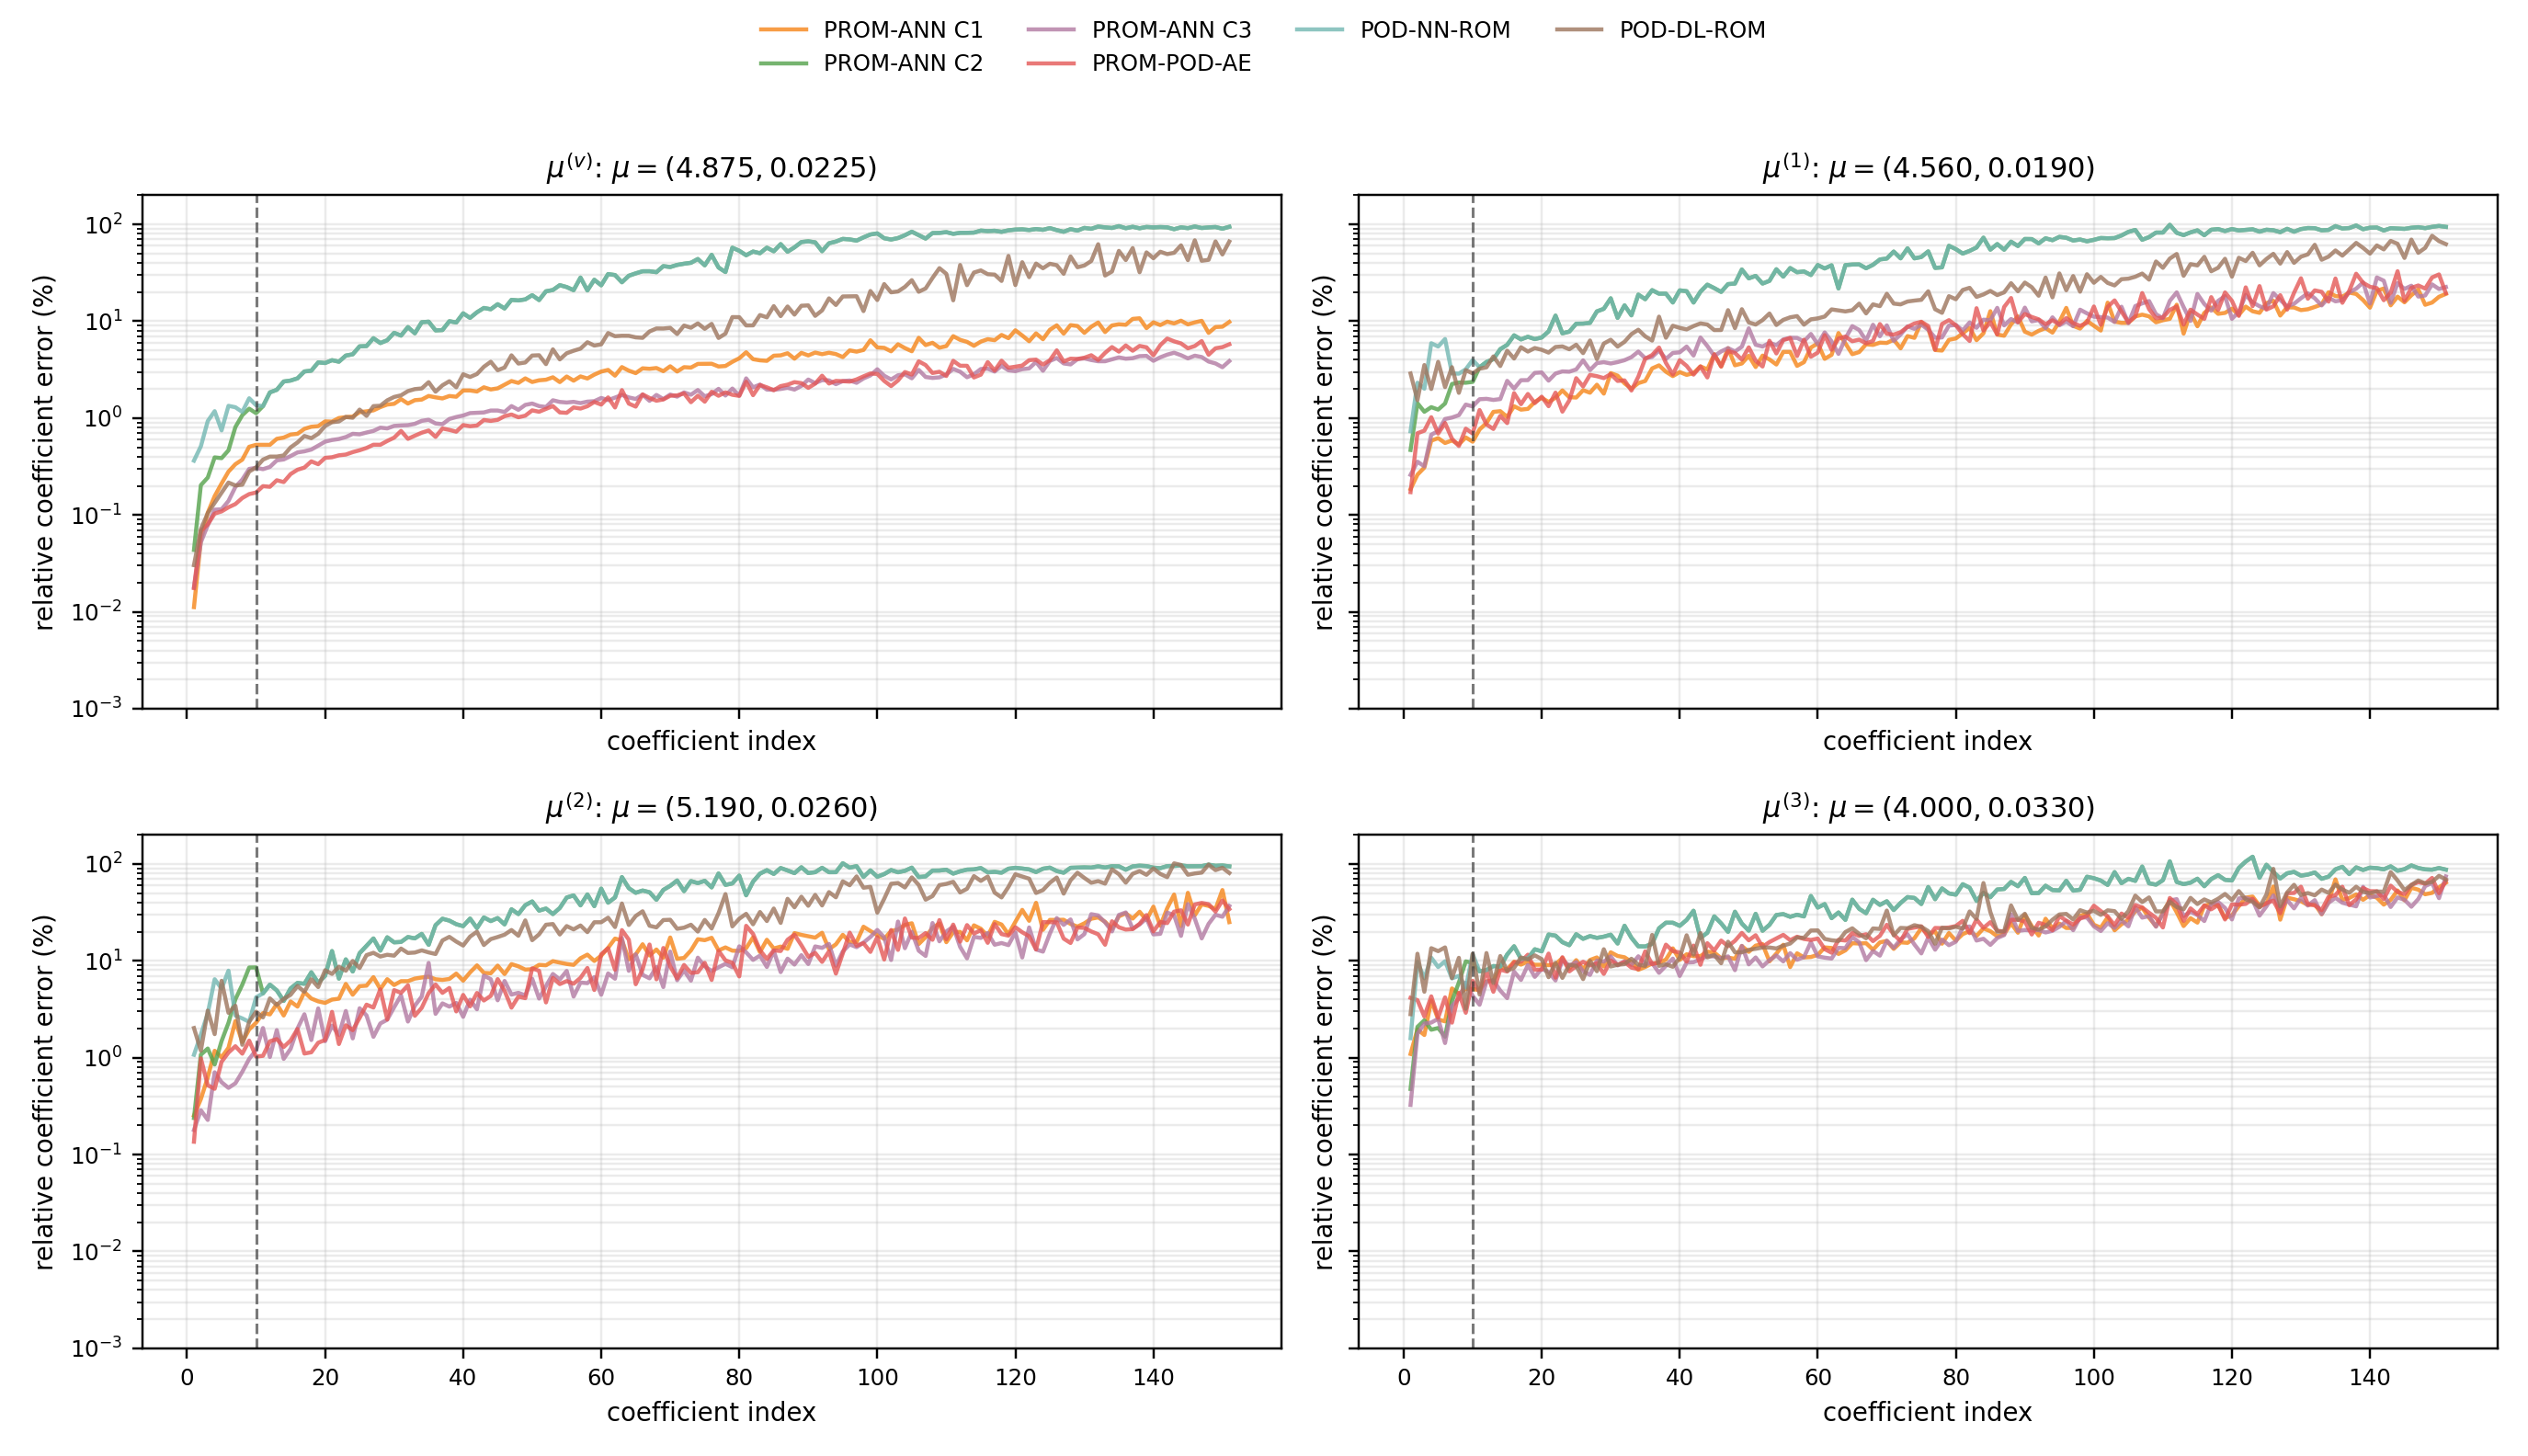
\includegraphics[width=0.98\textwidth]{Figures/prom_only/prom_only_coeff_rel_errors.png}
\caption{Baseline online per-coefficient relative errors against the \(n_{\mathrm{tot}}=151\) linear PROM coefficient
trajectory.  The vertical line marks coefficient 10.  The linear PROM itself is the reference and is not plotted.}
\label{fig:prom-coeff-rel-errors}
\end{figure}

The high-index coefficients often show large relative errors because their trajectory norms are small.  This does
not mean that each high-index coefficient dominates the state error.  It does show, however, that the map
\((\mu_1,\mu_2,t)\mapsto\q_{151}\) is data-limited in the baseline regime: the high-index tail is low energy but
still difficult to interpolate from only nine parameter trajectories.

\section{Effect of PROM Data Enrichment}
The enriched campaign tests whether the baseline degradation is primarily an architecture issue or a data-coverage
issue.  The architecture is kept fixed.  The basis \(\V_{151}\), validation points, online evaluation points, and
online PROM formulations are also unchanged.  Only the training coefficient data are expanded from nine PROM
trajectories to 45 PROM trajectories.

\begin{table}[H]
\centering
\caption{Training and validation coefficient errors before and after PROM data enrichment.  The validation set is
kept fixed when available, so the reduction measures generalization improvement rather than a change in evaluation
criterion.}
\label{tab:prom-enrichment-training}
\resizebox{0.9\textwidth}{!}{\begin{tabular}{lrr|rr|rr|rr}
\toprule
& \multicolumn{2}{c|}{Baseline (9)} & \multicolumn{2}{c|}{Early (9+8)} & \multicolumn{2}{c|}{Intermediate (9+18)} & \multicolumn{2}{c}{Enriched (9+36)} \\
Model & train $e_q$ (\%) & val. $e_q$ (\%) & train $e_q$ (\%) & val. $e_q$ (\%) & train $e_q$ (\%) & val. $e_q$ (\%) & train $e_q$ (\%) & val. $e_q$ (\%) \\
\midrule
PROM--ANN Case 1 & 1.130 & 1.251 & 0.742 & 0.825 & 0.512 & 0.557 & 0.360 & 0.374 \\
Master POD--NN--ROM (Case 2 tail source) & 2.601 & 4.391 & 0.983 & 1.625 & 0.580 & 0.814 & 0.435 & 0.555 \\
PROM--ANN Case 3 & 0.405 & 0.482 & 0.311 & 0.347 & 0.289 & 0.324 & 0.230 & 0.268 \\
PROM--POD--AE ($n_z=10$) & 0.106 & 0.127 & 0.087 & 0.098 & 0.084 & 0.095 & 0.054 & 0.074 \\
POD--DL--ROM ($n_z=10$) & 0.810 & 0.935 & 0.348 & 0.362 & 0.246 & 0.273 & 0.142 & 0.158 \\
\bottomrule
\end{tabular}
}
\end{table}

The strongest gain is obtained by the master Case 2/POD--NN map: its validation error decreases from
\(4.391\%\) to \(0.555\%\).  This is the clearest evidence that the previous difficulty was largely caused by the
sparsity of the nine-trajectory parameter training set, not by an intrinsic impossibility of learning the map in this
benchmark.  The POD--DL map also improves strongly, while the already accurate autoencoder still benefits.

\begin{table}[H]
\centering
\caption{Online state errors before and after PROM data enrichment.  The linear PROM row is unchanged and is shown
as the fixed reference accuracy level.}
\label{tab:prom-enrichment-online}
\resizebox{\textwidth}{!}{\begin{tabular}{lrrrrr|rrrrr}
\toprule
& \multicolumn{5}{c|}{Baseline (9 trajectories)} & \multicolumn{5}{c}{Enriched (9+36 trajectories)} \\
Model & $\mu^{(v)}$ & $\mu^{(1)}$ & $\mu^{(2)}$ & Mean & $\mu^{(3)}$ & $\mu^{(v)}$ & $\mu^{(1)}$ & $\mu^{(2)}$ & Mean & $\mu^{(3)}$ \\
\midrule
Linear PROM & 0.413 & 0.460 & 0.472 & 0.448 & 0.868 & 0.413 & 0.460 & 0.472 & 0.448 & 0.868 \\ 
PROM--ANN Case 1 & 0.409 & 0.520 & 0.683 & 0.537 & 1.584 & 0.411 & 0.459 & 0.469 & 0.446 & 0.868 \\ 
PROM--ANN Case 2 ($n=10$) & 1.013 & 1.427 & 1.670 & 1.370 & 1.898 & 0.435 & 0.477 & 0.496 & 0.469 & 0.872 \\ 
PROM--ANN Case 3 & 0.405 & 0.521 & 0.576 & 0.501 & 1.392 & 0.412 & 0.458 & 0.470 & 0.447 & 0.869 \\ 
PROM--POD--AE ($n_z=10$) & 0.408 & 0.539 & 0.607 & 0.518 & 1.978 & 0.412 & 0.459 & 0.471 & 0.447 & 0.871 \\ 
\midrule
POD--NN--ROM & 1.036 & 1.675 & 1.842 & 1.518 & 3.214 & 0.437 & 0.479 & 0.500 & 0.472 & 0.897 \\ 
POD--DL--ROM ($n_z=10$) & 0.489 & 1.398 & 1.463 & 1.116 & 3.728 & 0.414 & 0.460 & 0.473 & 0.449 & 0.868 \\ 
\bottomrule
\end{tabular}
}
\end{table}

\begin{figure}[H]
\centering

\includegraphics[width=0.98\textwidth]{Figures/prom_only/prom_enrichment_state_error_comparison.png}
\caption{Effect of PROM data enrichment on online state errors.  Left: mean error over the verification and two
off-grid in-domain points.  Right: extrapolatory point.}
\label{fig:prom-enrichment-state}
\end{figure}

After enrichment, all learned models are close to the linear PROM state accuracy at the reported points.  The most
important qualitative change is that the non-intrusive maps no longer behave as outliers: the enriched POD--NN--ROM
and POD--DL--ROM have state errors comparable to the intrusive learned PROMs.  For the extrapolatory point, the
enriched errors also collapse near the fixed linear PROM level, indicating that the exterior LHS samples provide
useful information in the expanded parameter region.

\begin{table}[H]
\centering
\caption{Online coefficient errors against the linear PROM teacher before and after PROM data enrichment.  Values
are relative Frobenius percentages in coefficient space.}
\label{tab:prom-enrichment-coeff}
\resizebox{0.9\textwidth}{!}{\begin{tabular}{lrrrrr|rrrrr}
\toprule
& \multicolumn{5}{c|}{Baseline (9 trajectories)} & \multicolumn{5}{c}{Enriched (9+36 trajectories)} \\
Model & $\mu^{(v)}$ & $\mu^{(1)}$ & $\mu^{(2)}$ & Mean & $\mu^{(3)}$ & $\mu^{(v)}$ & $\mu^{(1)}$ & $\mu^{(2)}$ & Mean & $\mu^{(3)}$ \\
\midrule
Linear PROM & 0.000 & 0.000 & 0.000 & 0.000 & 0.000 & 0.000 & 0.000 & 0.000 & 0.000 & 0.000 \\ 
PROM--ANN Case 1 & 0.295 & 0.593 & 1.297 & 0.729 & 2.923 & 0.066 & 0.057 & 0.089 & 0.070 & 0.178 \\ 
PROM--ANN Case 2 ($n=10$) & 2.440 & 3.361 & 3.906 & 3.236 & 4.257 & 0.377 & 0.357 & 0.433 & 0.389 & 0.583 \\ 
PROM--ANN Case 3 & 0.164 & 0.856 & 0.788 & 0.603 & 2.396 & 0.039 & 0.038 & 0.055 & 0.044 & 0.117 \\ 
PROM--POD--AE ($n_z=10$) & 0.140 & 0.773 & 0.929 & 0.614 & 4.394 & 0.041 & 0.041 & 0.059 & 0.047 & 0.151 \\ 
\midrule
POD--NN--ROM & 2.499 & 3.924 & 4.249 & 3.557 & 7.444 & 0.385 & 0.362 & 0.446 & 0.398 & 0.805 \\ 
POD--DL--ROM ($n_z=10$) & 0.814 & 3.129 & 3.225 & 2.389 & 8.639 & 0.108 & 0.099 & 0.130 & 0.112 & 0.240 \\ 
\bottomrule
\end{tabular}
}
\end{table}

\begin{figure}[H]
\centering

\includegraphics[width=0.98\textwidth]{Figures/prom_only/prom_enrichment_coeff_error_comparison.png}
\caption{Effect of PROM data enrichment on online coefficient errors.  The coefficient metric is stricter than the
state metric because it measures the entire \(151\)-coordinate trajectory against the linear PROM teacher.}
\label{fig:prom-enrichment-coeff}
\end{figure}

The coefficient table confirms the state-error interpretation.  The baseline POD--NN--ROM has an in-domain mean
coefficient error of \(3.557\%\) and \(7.444\%\) at the extrapolatory point.  After enrichment these decrease to
\(0.398\%\) and \(0.805\%\), respectively.  Case 2 with \(n=10\) improves similarly because it uses the same master
map for the injected tail.

\begin{figure}[H]
\centering
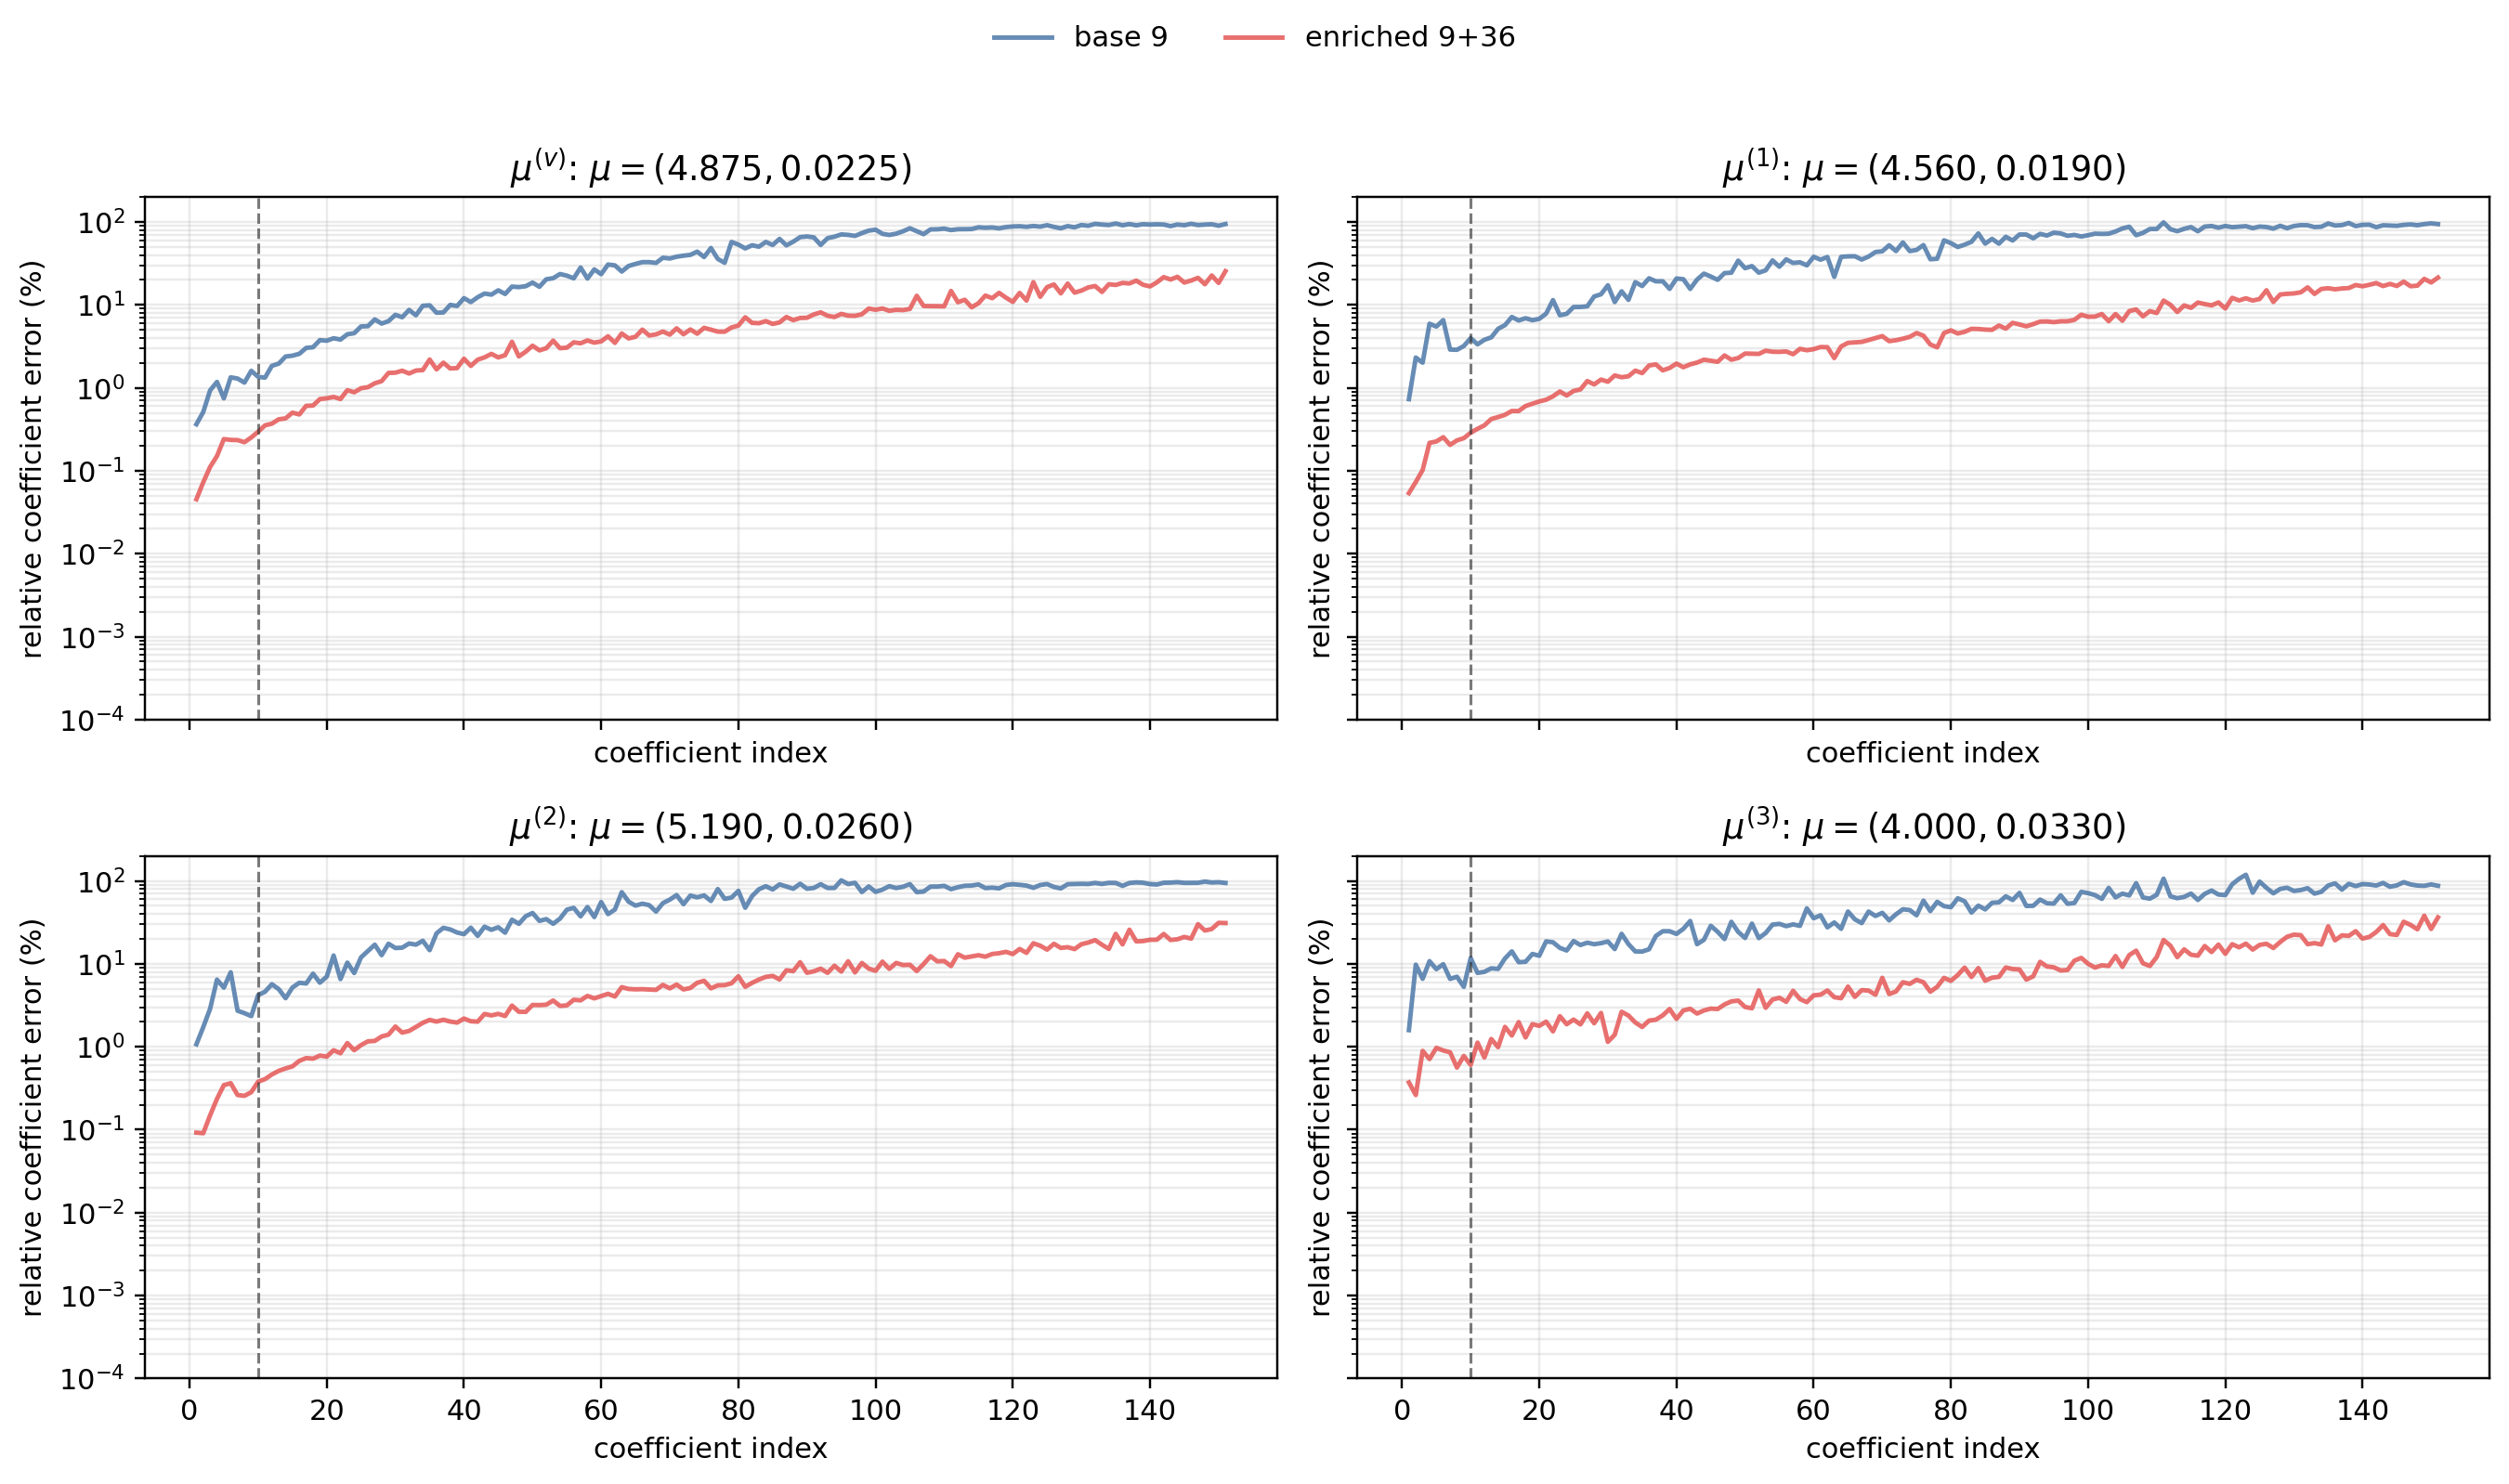
\includegraphics[width=0.98\textwidth]{Figures/prom_only/prom_enrichment_podnn_coeff_rel_errors.png}
\caption{Per-coefficient relative error of the direct POD--NN--ROM coefficient prediction before and after PROM data
enrichment.  The vertical line marks coefficient 10.  The plot uses the linear PROM coefficient trajectory as the
reference.}
\label{fig:prom-enrichment-podnn-coeff}
\end{figure}

Figure~\ref{fig:prom-enrichment-podnn-coeff} explains why enrichment matters.  With only nine trajectories, the
high-index tail has relative errors close to order one even when the global state error is moderate.  The enriched
training set reduces those tail errors over most coefficients, while preserving the already accurate leading
coefficients.  This is precisely the behavior needed by Case 2: the PROM solve can recover the primary coordinates,
but the residual still sees the injected secondary tail.

\section{Conclusions}
The PROM-only study supports the following conclusions.
\begin{enumerate}
  \item The fixed MLSPG-sensitive linear PROM provides a reproducible coefficient teacher and state-accuracy
  reference for this benchmark.
  \item With only nine training trajectories, direct parameter--time prediction of all 151 coefficients is the
  limiting task.  This affects both the POD--NN--ROM and the Case 2 injected tail.
  \item Solving more primary coordinates in Case 2 can help, but the residual solve remains coupled to the predicted
  secondary tail; therefore tail accuracy is still important.
  \item PROM data enrichment changes the picture substantially.  Keeping the architecture and basis fixed, the
  9+36 PROM trajectory set reduces validation and online coefficient errors and brings the learned state errors close
  to the linear PROM level.
  \item The next step should introduce residual sampling only after this PROM-level behavior is locked down, so that
  any additional error can be attributed to the sampled online residual rather than to the learned coefficient maps.
\end{enumerate}

\end{document}
